\documentclass[12pt,a4paper]{article}
%police
\usepackage[utf8]{inputenc}
\usepackage[T1]{fontenc}
\usepackage[french]{babel}

\usepackage[tc]{titlepic}

\usepackage{adjustbox}
\usepackage{graphicx}
\usepackage{layout}
\usepackage{fancyhdr}
\usepackage{eurosym}
\usepackage{multirow}
\usepackage{float}

\usepackage{hyperref}

\usepackage{geometry}
\geometry{margin=1.2in}

\pagestyle{fancy}
\fancyhead{}
\renewcommand{\headrulewidth}{0pt}
\lfoot{PLT - BALACHANDRAN Chirojean - FAUJEAU François}
\cfoot{}
\rfoot{\thepage}

\begin{document}

\begin{titlepage}

\newcommand{\HRule}{\rule{\linewidth}{0.5mm}} % Defines a new command for the horizontal lines, change thickness here

\begin{minipage}{0.4\textwidth}
\begin{flushleft} \large

\includegraphics[width=0.5\textwidth]{Logo_ENSEA.jpg} 
\end{flushleft}
\end{minipage}
~
\begin{minipage}{0.57\textwidth}
\begin{flushright} \large
FAUJEAU François \textsc{} \\
BALACHANDRAN Chirojean\textsc{} \\
3A IS\textsc{} \\
\end{flushright}
\end{minipage}\\[1cm]

\centering

\HRule \\[0.5cm]
{ \huge \bfseries PROJET CIVILIZATION}\\[0.3cm]% Title of your document
Rapport du projet logiciel transversal \textsc{} \\[0.5cm]
\HRule \\[3cm]


\includegraphics[width=1\textwidth]{map.png}\\[3.5cm]


\begin{flushleft}
Année scolaire: 2018-2019
\end{flushleft}
\end{titlepage}


\newpage

\tableofcontents
\thispagestyle{empty}
\setcounter{page}{0}

\newpage

\section{Présentation générale}

\subsection{Archétype}

Le but de notre projet logiciel transversal est de créer une version très simplifiée du jeu civilization. Ce jeu est un jeu de stratégie tour par tour où l'objectif d'un joueur est de développer un empire en choississant une civilisation au choix parmi plusieurs. 

\begin{figure}[!ht]
    \centering
    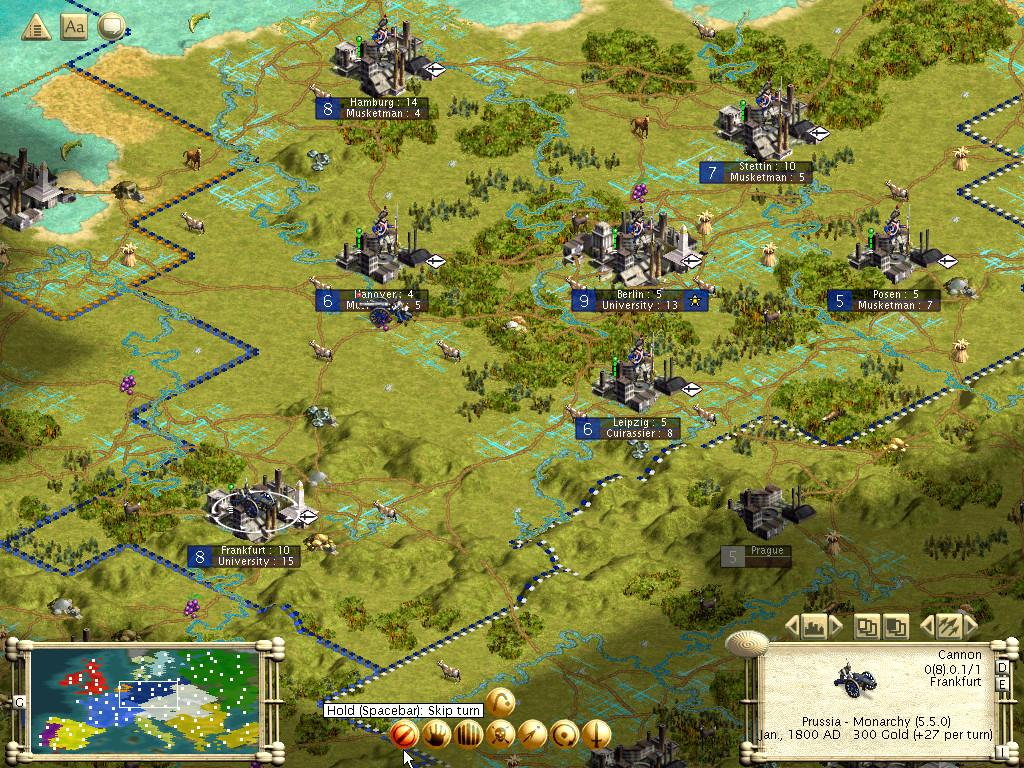
\includegraphics[width=0.7\textwidth]{civ3.png}
     \caption{Image d'un gameplay de civilization 3}
\end{figure}

\subsection{Règles du jeu}

Le but pour chaque joueur est de développer un empire avec la civilisation romaine. Pour cela, le joueur doit améliorer et gérer ses ressources (mines d'or, terres agricoles) ainsi que ses bâtiments (caserne et palais). \\
Nous avons choisi que chaque joueur pourrait seulement utiliser la civilisation romaine. Chaque empire permet de créer différents bâtiments : 
\begin{enumerate}
    \item Le palais : bâtiment principal de l'empire. Son niveau correspond au niveau de l'empire. Plus sont niveau est élevé et plus il est possible d'améliorer les autres bâtiments et unités.
    \item La caserne : permet de former des soldats. Quand le niveau de la caserne augmente, le niveau des troupes formées et le nombre des troupes qui peuvent être formées augmentent. Il y aura quatre types d'unités de combat : un cavalier, un épéiste, un archer et une catapulte. A la création d'une unité, le joueur choisira si elle est créée pour défendre l'empire ou si elle peut se déplacer sur la carte de jeu.
    \item Ressources : le joueur possèdera trois types de ressources à savoir les mines d'or, la réserve de bois et les terres agricoles. Quand le niveau d'une ressource augmente, la capacité de stockage de cette ressource et la quantité produite sont augmentées.
\end{enumerate}
Pour améliorer les bâtiments, il faudra que le joueur dépense une certaine quantité de bois et d'or et pour la formation de soldats une certaine quantité de récoltes agricoles et d'or.\\
Pour développer son empire plus rapidement il est possible d'en combatre un autre (détenu soit par l'IA, soit par un joueur) ou de s'en défendre. En effet, en cas de victoire l'empire victorieux reçoit une partie des ressources de l'empire adverse et un bonus de victoire. L'empire qui a perdu recupère, lui, un faible bonus de défaite. \\Le système de combat est le suivant. 
Chacun leur tour, les joueurs pourront décider de : 
\begin{itemize}
    \item se déplacer pour se rapprocher du combat.
    \item choisir qu'un soldat en attaque un autre s'il est dans sa zone d'action.
\end{itemize}
Un combat se termine lorsque tous les soldats d'un joueur sont éliminés. 
\\Dans notre jeu, un tour correspond à une action: une amélioration de bâtiment, la formation d'une unité, son déplacement.\\

\subsection{Ressources}

Voici les différentes ressources (images, textures, sprites) utilisées pour le développement du jeu. Pour créer les cartes de jeu nous utiliserons le logiciel Tiled Map Editor en mode isométrique. 

\begin{figure}[!ht]
    \centering
    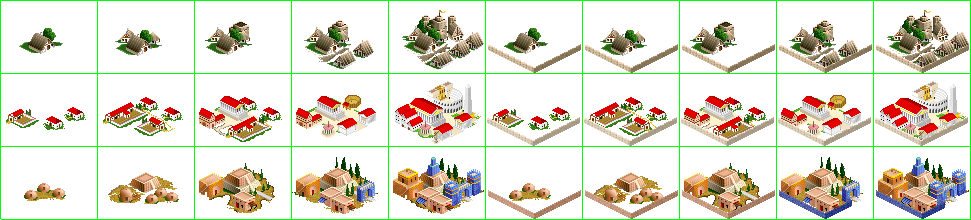
\includegraphics[width=0.7\textwidth]{ressources/cities2.png}
     \caption{Bâtiments de la civilisation romaine en fonction des niveaux}
\end{figure}

\begin{figure}[!ht]
    \centering
    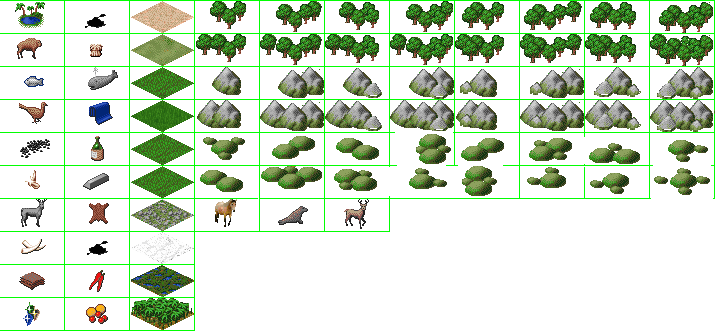
\includegraphics[width=0.7\textwidth]{ressources/Terrain.png}
     \caption{textures pour la création de la map}
\end{figure}
\newpage
\begin{figure}[!ht]
    \centering
    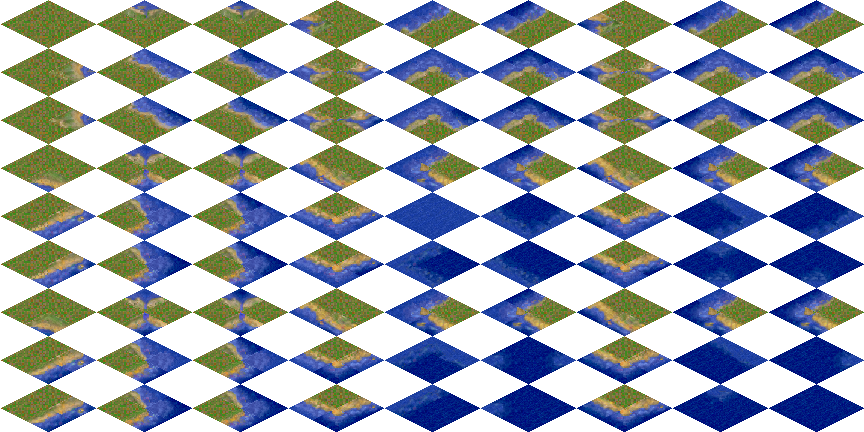
\includegraphics[width=0.7\textwidth]{ressources/ocean.png}
     \caption{textures pour la mer sur la map}
\end{figure}

\begin{figure}[!ht]
    \centering
    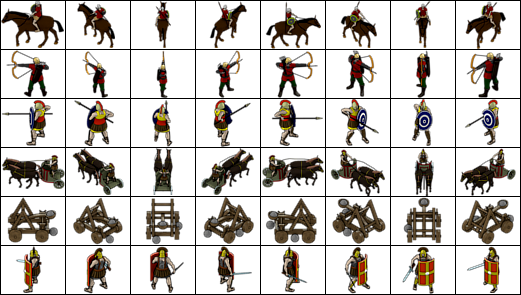
\includegraphics[width=0.7\textwidth]{ressources/Units.png}
     \caption{images des unités de combats}
\end{figure}


\end{document}